\begin{center}
  \vspace*{25pt}
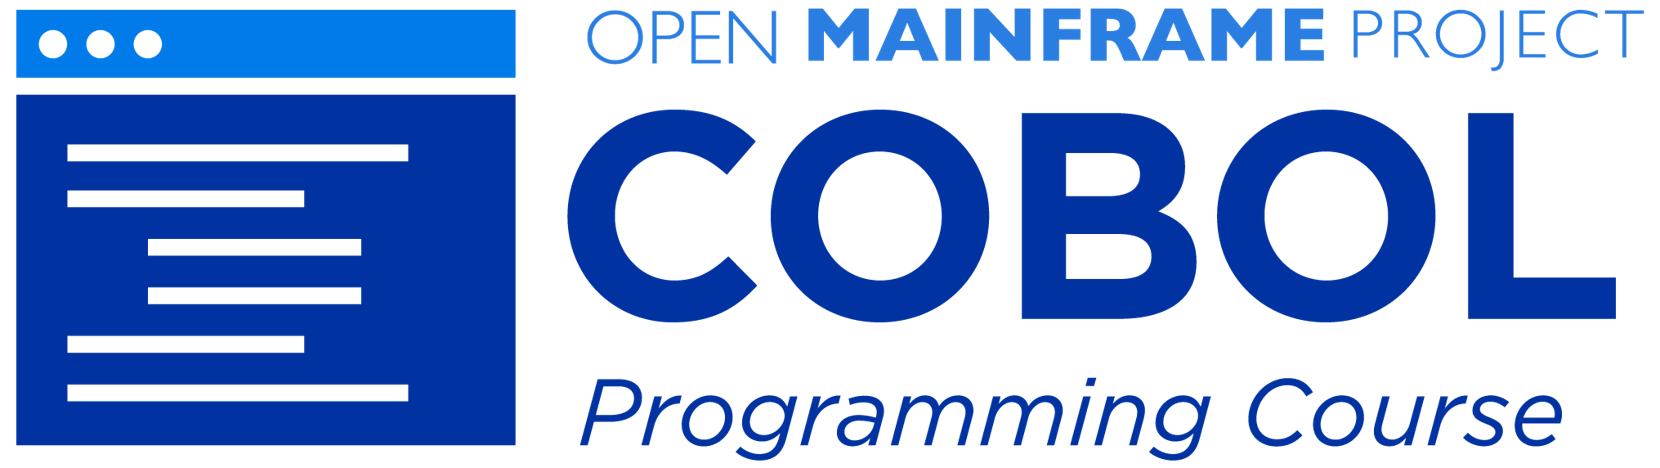
\includegraphics{Images/COBOL-Programming-Course.png}
\hypertarget{cobol-programming-course-1}{%
\section*{
  \\[35pt]
  \Huge Curso de Programación en COBOL 1 \\[10pt]
  \Huge Introducción \\[15pt]
  \Large Version 3.0.0}\label{cobol-programming-course-1}}
\end{center}

\pagebreak
\hypertarget{copyright}{%
\section*{Copyright}{
  \normalsize COBOL Programming Course is licensed under Creative Commons 
  Attribution 4.0 International. To view a copy of this license, visit 
  \href{https://creativecommons.org/licenses/by/4.0}{https://creativecommons.org/licenses/by/4.0}. \\[10pt]
  Copyright Contributors to the Open Mainframe Project's COBOL Programming Course}\label{copyright}}
\pagebreak

\hypertarget{preface}{%
\section*{Prefacio}\label{preface}}

\hypertarget{abstract}{%
\subsection*{Resumen}\label{abstract}}

Solamente un lenguaje de programación ha sido diseñado específicamente 
para aplicaciones empresariales, Common Business-Oriented Language, COBOL.
En la actualidad COBOL se mantiene tan relevante como antes, manejando
\$3 billones de dólares en comercio cada día.

Esta publicación está dirigida a principiantes que buscan aprender
de COBOL. Describe como trabajar con COBOL usando herramientas modernas
como Visual Studio Code, y extensiones como Zowe para Visual Studio Code
y z Open Editor. Además describe como escribir, probar, ejecutar y 
depurar programas escritos en COBOL.

\hypertarget{authors}{%
\subsection*{Autores}\label{authors}}

\textbf{Michael Bauer} Es un desarrollador líder para el desarrollo
del flujo de valor de Open Mainframe en Broadcom. Y dirige la iniciativa
de código abierto de Zowe. El entorno de desarrollo Zowe es una popular
herramienta para interactuar con z/OS, y abre la oportunidad a los 
trabajos hechos sobre sistemas Mainframe de usar la metodología DevOps
y sus prácticas. Mike lidera el equipo de desarrollo de la linea de comandos
de Zowe (Zowe CLI), quienes crearon y recientemente dieron a conocer el
explorador de Zowe, que es una extension para Visual Studio Code.
El tambien es un reconocido orador y blogger, y ha realizado talleres
interactivos alrededor del mundo para aquellos interesados en incorporar
los sistemas Mainframe en sus actividades de DevOps.

\textbf{Ahmed Eid} is a computer engineering student from Egypt. He was 
a mentee for the Open Mainframe Project 2021 Summer Mentorship under the 
COBOL Programming Course, helping to improve the content of the course.

\textbf{Zeibura Kathau} is a technical writer for the Mainframe DevOps
value stream at Broadcom. He works on the open-source projects Che4z and 
Code4z, which are IDE extension packages for mainframe developers. He has 
8 years of experience in the Information Technology field.

\textbf{Makenzie Manna} is an IBM Redbooks Project Leader in the United
States. She has 3 years of experience in the Computer Science Software
Development field. She holds a Master's degree in Computer Science
Software Development from Marist College. Her areas of expertise include
mathematics, IBM Z and cloud computing.

\textbf{Paul Newton} is a Consulting IT Specialist in the United States.
He has 40 years of experience in the Information Technology field. He
holds a degree in Information Systems from the University of Arizona.
His areas of expertise include IBM Z, z/OS, and LinuxONE. He has written
extensively on implementation of z/OS based technology.

\textbf{Jonathan Sayles} is a technical educator at IBM, where he
conducts presentations, seminars and training courses, as well as
producing educational materials. His more than 40 years in the IT
education and computer industries encompass work within both academic
and corporate development organizations. He has also been engaged as a
software developer/designer/consultant, educator, and author, with a
focus on relational database, IDE, and object technologies. In addition
to authoring/publishing 16 books, Jon has written and published more
than 150 articles in technical journals, and served as technical editor
for several IT magazines. He is also co-author of IBM Redbook
publications Transitioning: Informix 4GL to Enterprise Generation
Language (EGL), SG24-6673 and z/OS Traditional Application Maintenance
and Support, SG24-7868.

\textbf{Hartanto Ario Widjaya} is a computer science student from 
Singapore Management University. He was a mentee for the Open Mainframe 
Project 2021 Summer Mentorship under the COBOL Programming Course, 
helping to improve the content of the course with various additions and 
assisting new learners to incorporate COBOL as a part of their tech 
toolkit.

\textbf{William Yates} is a Software engineer working for IBM UK. For
the majority of his career he has working on the CICS TS product mainly
as a software tester and now as Test Architect. He has delivered
technical content for many Redbooks, video courses and at conferences
around the world. He is also one of the leaders of the Galasa project,
building an open source integration test framework for hybrid cloud
applications available at \href{https://galasa.dev/}{https://galasa.dev}.

\hypertarget{acknowledgements}{%
\subsection*{Agradecimientos}\label{acknowledgements}}

Especial gracias a quienes participaron en la residencia para darle forma a esta publicación.

\begin{itemize}
\item
  Dr.~Tak Auyeung, Profesor en American River College
\item
  Jeffrey Bisti, Arquitecto en el ecosistema Z, IBM
\item
  Ilicena Elliott, Especialista de IT II, Departamento de recursos humanos
\item
  Martin Keen, Técnico de servicios en contenido, IBM
\item
  Sudharsana Srinivasan, Influencer coordinador del programa Z, IBM
\item
  Suzy Wong, Especialista en tecnologías de la información, DMV
\item
  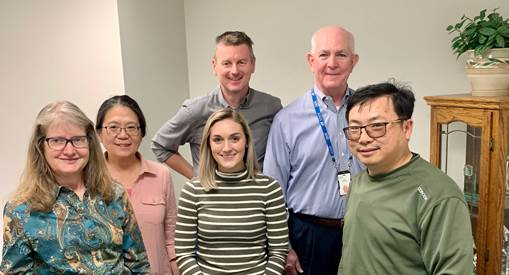
\includegraphics{Images/image004.jpg}
\end{itemize}

De izquierda a derecha: Ilicena, Suzy, Makenzie, Martin, Paul, y Tak
\pagebreak
